% header
\documentclass[10pt,a4paper]{article}

\usepackage[utf8]{inputenc}
\usepackage{hyperref}
\usepackage{amssymb}
\usepackage{amsmath}
\usepackage{listings}
\usepackage{graphicx}

% the document
\begin{document}

\title{Worksheet $2$\\
\small{Practical Lab Numerical Computing}}
\author{Andrii Lischishin \and Lars Schleithoff \and Hendrik Kleikamp}
\date{\today}
\maketitle

\section*{Task 1}

\begin{center}
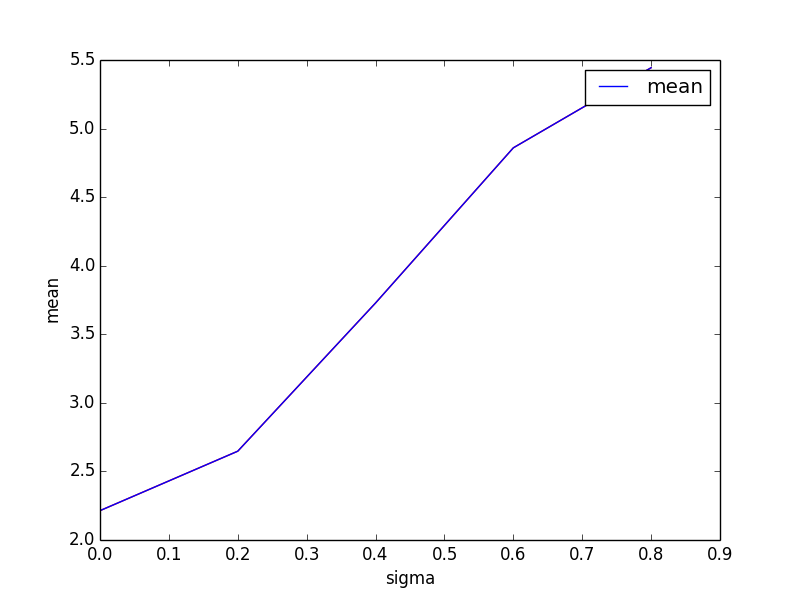
\includegraphics[scale=0.5]{task_1.png}		
\end{center}	

\section*{Task 2}

\begin{center}
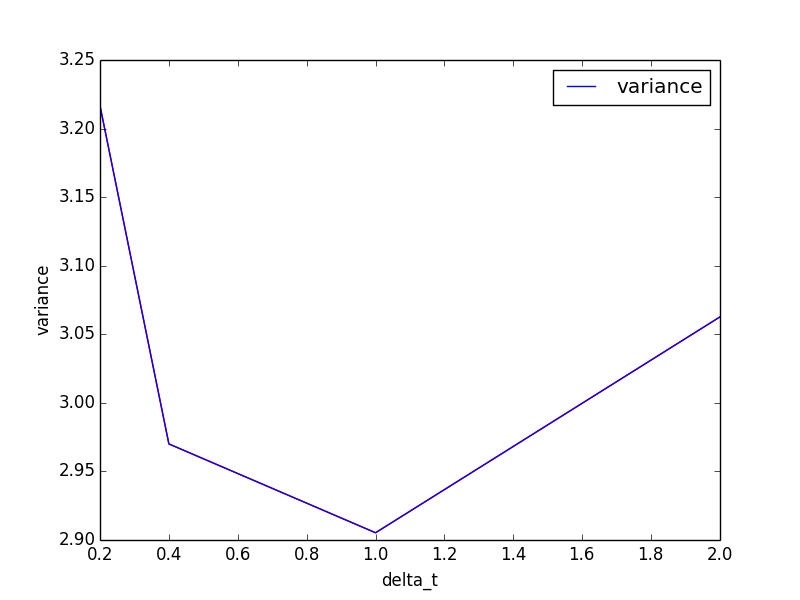
\includegraphics[scale=0.5]{task_2.png}		
\end{center}	

\section*{Task 3}
To prove that
\[
\mathbb{E}[V_{call}(S_T,0)]=S(0)\exp(\mu T)\Phi(\sigma\sqrt{T}-\chi)-K\Phi(-\chi)
\]
we use that by change-of-variable with $t:=-t$ we get
\begin{eqnarray}
&&\mathbb{E}[V_{call}(S_T,0)] \notag\\
&=&\frac{1}{\sqrt{2\pi}}\int_{\chi}^{\infty}\left(S(0)\exp\left((\mu-\frac{1}{2}\sigma^2)\cdot T+\sigma\sqrt{T}s\right)-K\right)\exp\left(-\frac{s^2}{2}\right)ds \notag\\
&=&\frac{1}{2\pi}\int_{\chi}^{\infty}\left(S(0)\exp\left((\mu-\frac{1}{2}\sigma^2)\cdot T+\sigma\sqrt{T}s\right)\right)\exp\left(-\frac{s^2}{2}\right)ds-K\frac{1}{2\pi}\int_{\chi}^{\infty}\exp\left(-\frac{t^2}{2}\right)dt \notag\\
&=&\Psi-K\frac{1}{2\pi}\int_{-\infty}^{-\chi}\exp\left(-\frac{t^2}{2}\right)dt \notag\\
&=&\Psi-K\Phi(-\chi) \notag
\end{eqnarray}
with
\[
\Psi:=\frac{1}{2\pi}\int_{\chi}^{\infty}\left(S(0)\exp\left((\mu-\frac{1}{2}\sigma^2)\cdot T+\sigma\sqrt{T}s\right)\right)\exp\left(-\frac{s^2}{2}\right)ds.
\]
Now we prove that
\[
\Psi=S(0)\exp(\mu T)\Phi(\sigma\sqrt{T}-\chi).
\]
Again, we use a change-of-variable $z:=t+\sigma\sqrt{T}$ and get
\begin{eqnarray}
&&\frac{1}{\sqrt{2\pi}}\exp\left(\frac{\sigma^2}{2}T\right)\int\limits_{-\infty}^{\sigma\sqrt{T}-\chi}\exp\left(-\frac{t^2}{2}\right)dt \notag\\
&=&\frac{1}{\sqrt{2\pi}}\exp\left(\frac{\sigma^2}{2}T\right)\int\limits_{\chi-\sigma\sqrt{T}}^{\infty}\exp\left(-\frac{t^2}{2}\right)dt \notag\\
&=&\frac{1}{\sqrt{2\pi}}\exp\left(\frac{\sigma^2}{2}T\right)\int\limits_{\chi}^{\infty}\exp\left(-\frac{(\sigma\sqrt{T}-z)^2}{2}\right)dz \notag\\
&=&\frac{1}{\sqrt{2\pi}}\int\limits_{\chi}^{\infty}\exp\left(-\frac{z^2}{2}+z\sigma\sqrt{T}\right)dz. \notag
\end{eqnarray}
We have
\begin{eqnarray}
\Psi&=&\frac{1}{\sqrt{2\pi}}S(0)\exp\left((\mu-\frac{\sigma^2}{2})\cdot T\right)\int_{\chi}^{\infty}\exp\left(-\frac{s^2}{2}+\sigma\sqrt{T}s\right)ds \notag\\
&=&S(0)\exp(\mu T)\exp\left(-\frac{\sigma^2}{2}T\right)\frac{1}{\sqrt{2\pi}}\int_{\chi}^{\infty}\exp\left(-\frac{s^2}{2}+\sigma\sqrt{T}s\right)ds \notag\\
&=&S(0)\exp(\mu T)\frac{1}{\sqrt{2\pi}}\exp\left(-\frac{\sigma^2}{2}T\right)\exp\left(\frac{\sigma^2}{2}T\right)\int\limits_{-\infty}^{\sigma\sqrt{T}-\chi}\exp\left(-\frac{s^2}{2}\right)ds \notag\\
&=&S(0)\exp(\mu T)\Phi(\sigma\sqrt{T}-\chi). \notag
\end{eqnarray}

\section*{Task 4}

\begin{center}
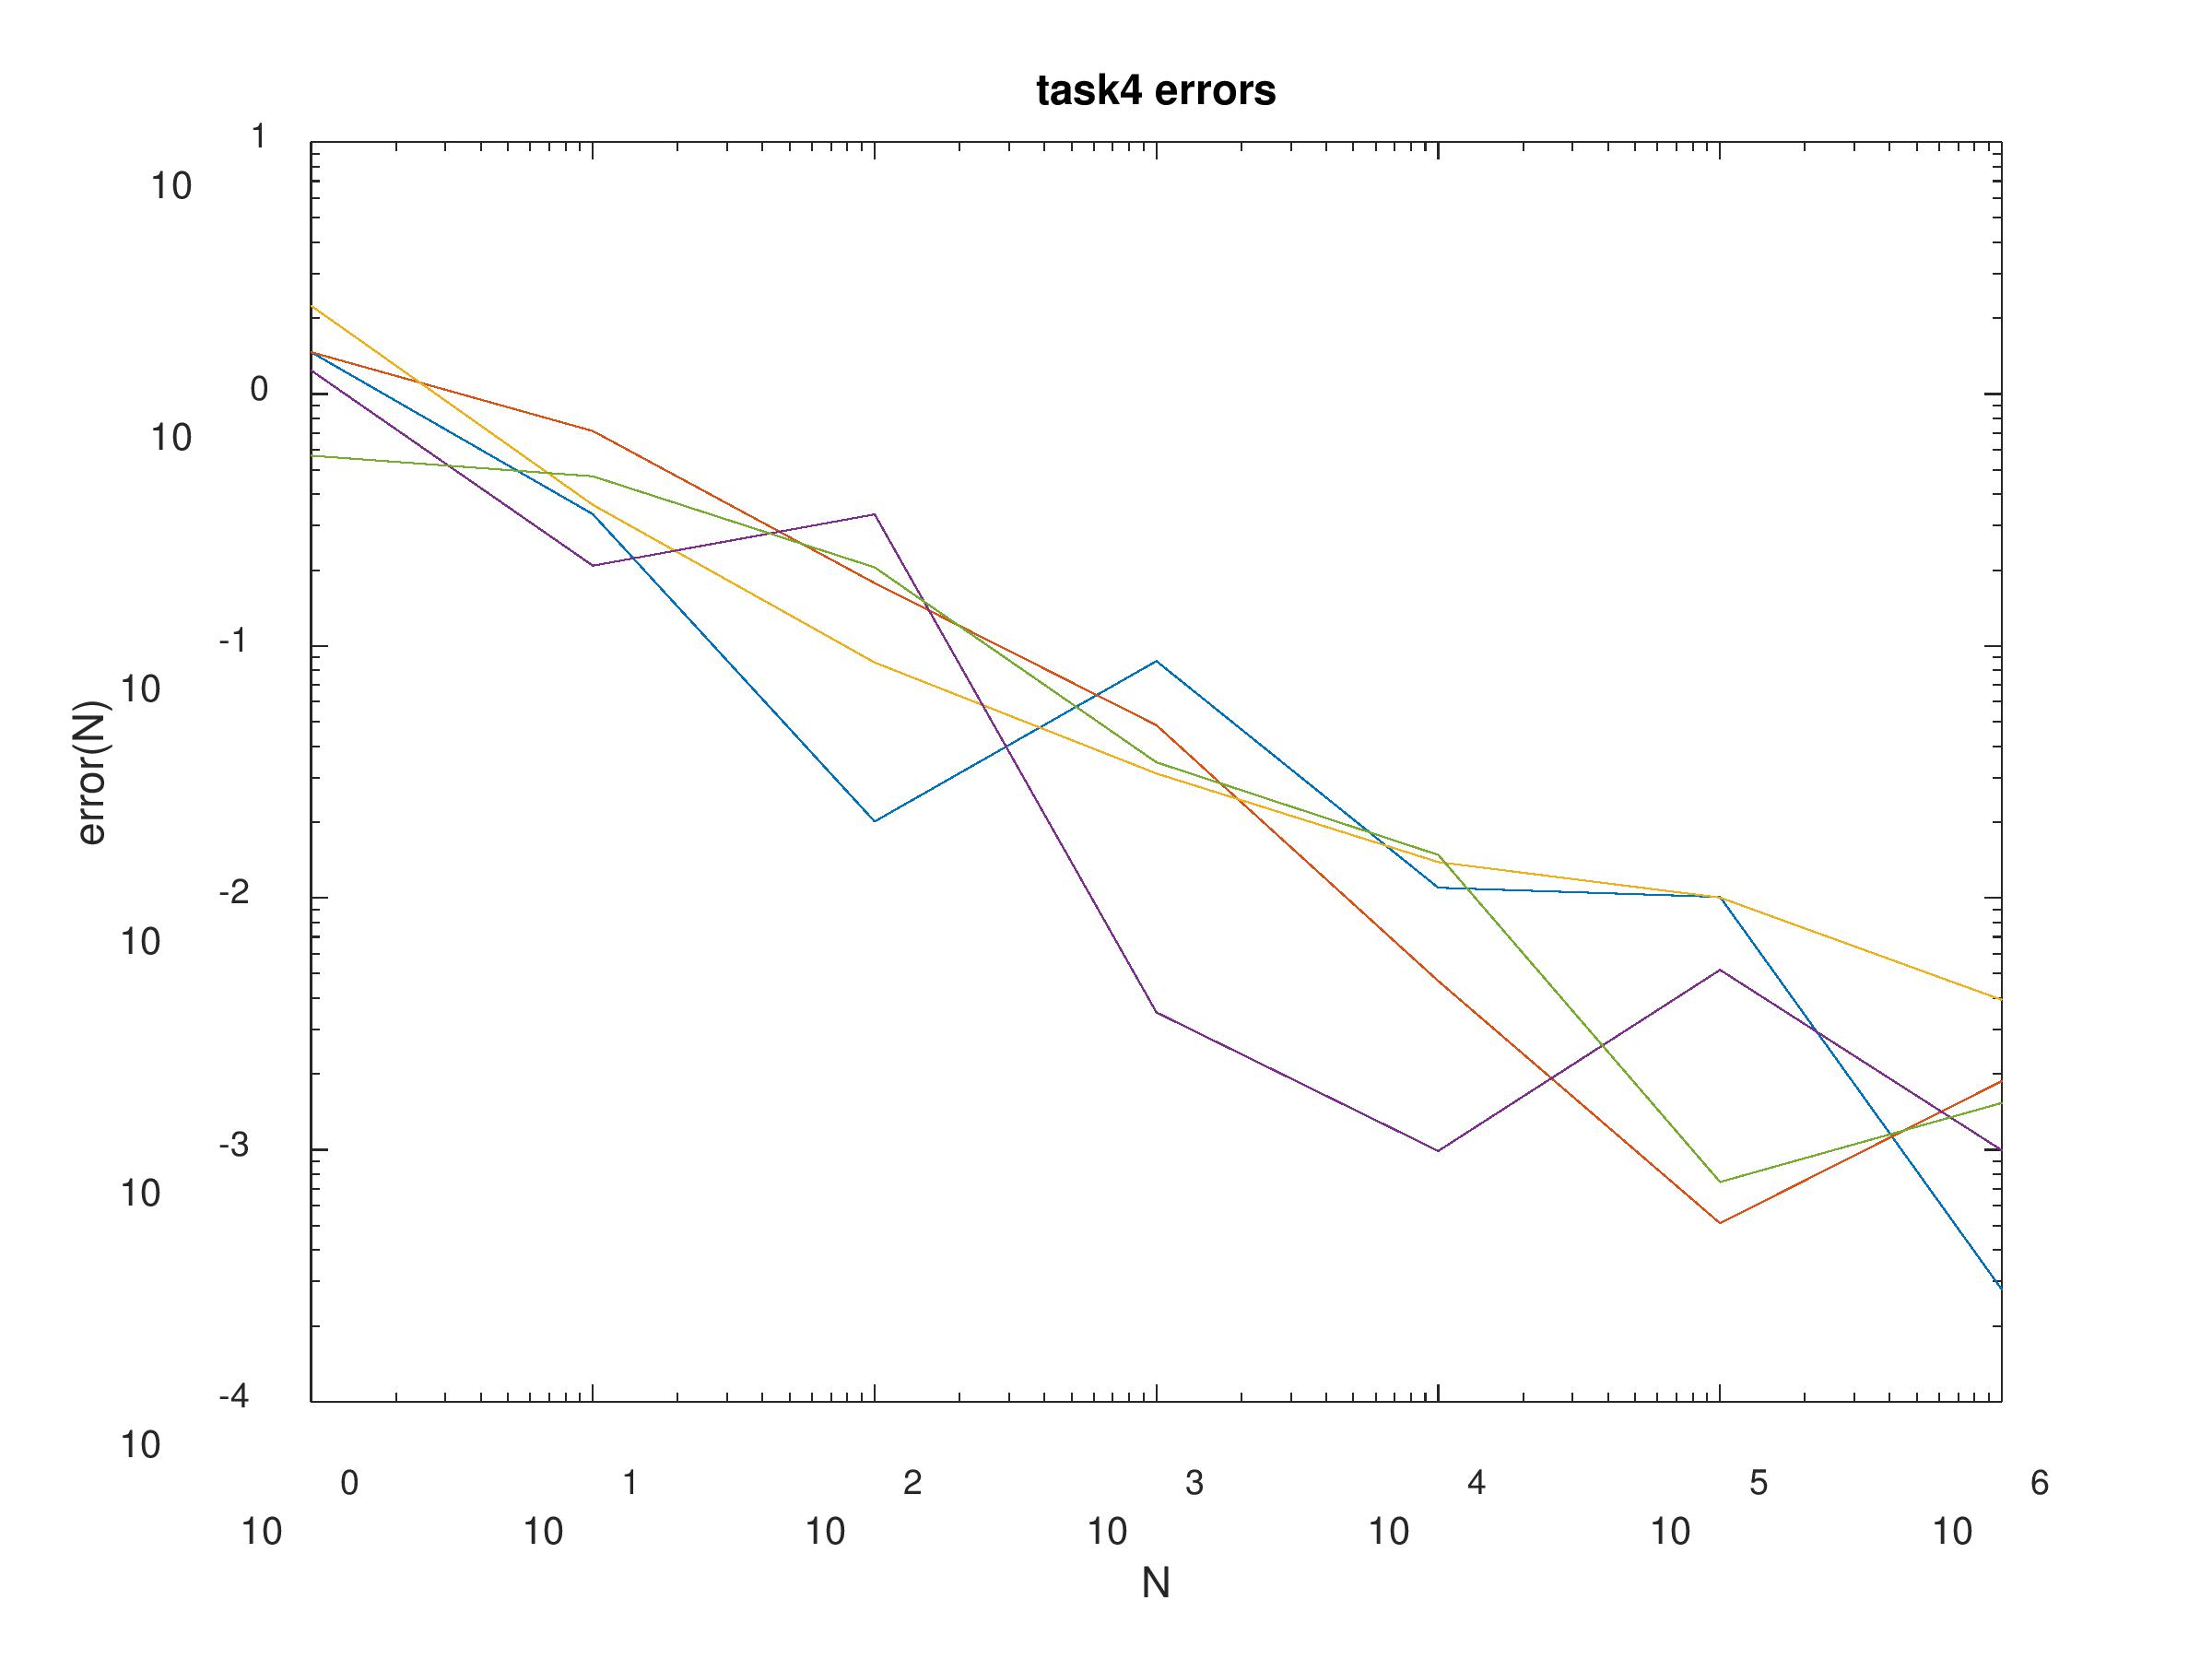
\includegraphics[scale=0.3]{task4.jpg}		
\end{center}	

\section*{Task 5}
We have $\Phi^{-1}(0)=-\infty$ and $\Phi^{-1}(1)=\infty$ where $\Phi^{-1}:(0,1)\to(-\infty,\infty)$ is the inverse cumulative distribution function. As an integral of a positive continious function, $\Phi$ is a bijection, continious and differentiable. That means $\Phi$ is a diffeomorphism. $\Phi^{-1}$ is also differentiable, so we can use the transformation theorem with the change-of-variable $t=\Phi(s)$. We have $|\det(D\Phi(s))|=\frac{1}{\sqrt{2\pi}}\exp(-\frac{s^2}{2})$ and
\begin{eqnarray}
&&\int_0^1 f(\Phi^{-1}(t))dt \notag\\
&=&\int_{\Phi^{-1}(0)}^{\Phi^{-1}(1)}f(\Phi^{-1}(\Phi(s)))\cdot|\det(D\Phi(s))|ds \notag\\
&=&\int_{-\infty}^{\infty}f(s)\frac{1}{\sqrt{2\pi}}\exp\left(-\frac{s^2}{2}\right)ds \notag\\
&=&\frac{1}{\sqrt{2\pi}}\int_{-\infty}^{\infty}f(s)\exp\left(-\frac{s^2}{2}\right)ds \notag
\end{eqnarray}
what proves formula (7).

\section*{Task 6}

In case of the trapezoidal-rule, the set of nodes of level $l$ is a subset of the nodes of level $l+1$. Furthermore, the $2^l$ additional values lay exactly half way in between the nodes of level $l$. (Except for the first and the last node, which lie half way in between 0 and the first node of level $l$ and in between the last node of level $l$ and the end of the interval.) 

\section*{Task 7}

In case of the Gauß-Legendre Quadrature, the nodes of level $l$ are not a subset of the nodes of level $l+1$. At the edges of the interval, the nodes are denser. According to Satz 1.18 from Einführung in die Grundlagen der Numerik, node $x_i^{(N_l)}$ from level $l$ lays between the nodes $x_i^{(N_{l+1})}, x_{i+1}^{(N_{l+1})}$ from level $l+1$.

The nodes are the roots of a three-term-recurrence relation of the form $p_{n+1}(t)=(t-\alpha_n)p_n(t)-\beta_n^2p_{n-1}(t)$, $n \geq 0$. 
The roots are the eigenvalues of a tridiagonal $(N_l \times N_l)$-dimensional matrix of the form

\begin{align*}
\begin{bmatrix}
\alpha_0 &  \beta_1  & 0 & ... & ... & ... \\
\beta_1 & \alpha_1 & \beta_2 & ... & ... & ... \\
 0  & \beta_2 & a_2 & \beta_3 & ... & ... \\
0   & ... & ... & ... & ... & 0 \\
... & ... &  0  & \beta_{N_l-2} & \alpha_{N_l-2} & \beta_{N_l-1}  \\
... & ... & ... & 0  & \beta_{N_l-1} & \alpha_{N_l-1} \\
\end{bmatrix}
\end{align*}



The weights are the first entry of the eigenvectors to the eigenvalues calculated for the nodes. Alternitavely, they can be recieved by taking $\Lambda_{n+1}(x_i)$ of the Christoffel-function, with $x_i, i=1,...,n$ nodes. 



\section*{Task 8}

The Clenshaw-Curtis Quadrature rule uses nested nodes, the nodes of each level are a subset of the nodes of higher levels. Similarly to Gauß-Legendre quadrature, the number of nodes is higher at the edges of the integral. 

\section*{Task 9}

\begin{center}
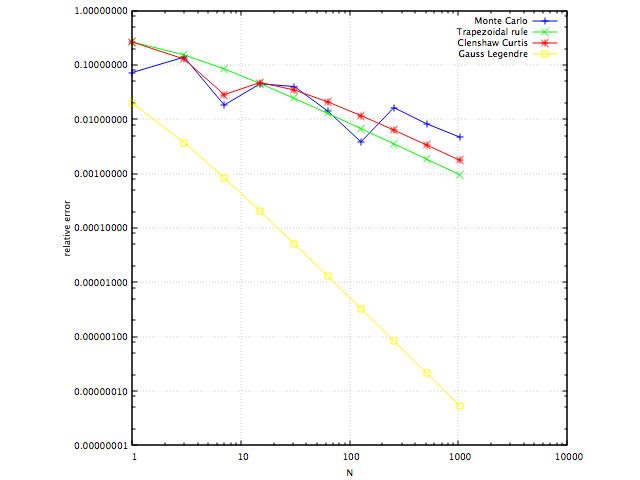
\includegraphics[scale=0.5]{relative_errors_K0.png}		
\end{center}	

\section*{Task 10}

\begin{center}
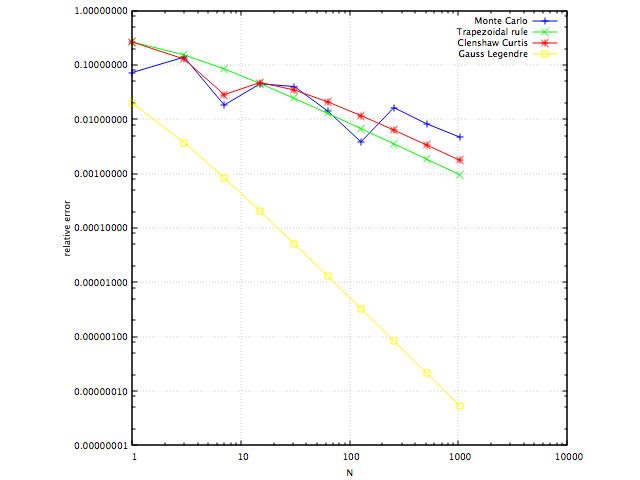
\includegraphics[scale=0.5]{relative_errors_K0.png}		
\end{center}	

\begin{center}
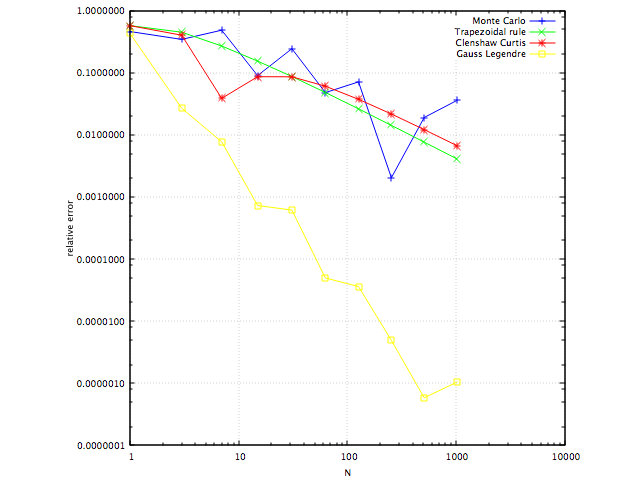
\includegraphics[scale=0.5]{relative_errors_K10.png}		
\end{center}	

\end{document}